%%%%%%%%%%%%%%%%%%%%%%%%%%%%%%%%%%%%%%%%%
% baposter Landscape Poster
% LaTeX Template
% Version 1.0 (11/06/13)
%
% baposter Class Created by:
% Brian Amberg (baposter@brian-amberg.de)
%
% This template has been downloaded from:
% http://www.LaTeXTemplates.com
%
% License:
% CC BY-NC-SA 3.0 (http://creativecommons.org/licenses/by-nc-sa/3.0/)
%
%%%%%%%%%%%%%%%%%%%%%%%%%%%%%%%%%%%%%%%%%

%----------------------------------------------------------------------------------------
%	PACKAGES AND OTHER DOCUMENT CONFIGURATIONS
%----------------------------------------------------------------------------------------

\documentclass[landscape,a2paper,fontscale=0.54]{baposter} % Adjust the font scale/size here

\usepackage{graphicx} % Required for including images
\graphicspath{{figures/}} % Directory in which figures are stored

\usepackage{amsmath} % For typesetting math
\usepackage{amssymb} % Adds new symbols to be used in math mode

\usepackage{booktabs} % Top and bottom rules for tables
\usepackage{enumitem} % Used to reduce itemize/enumerate spacing
\usepackage{palatino} % Use the Palatino font
\usepackage[font=small,labelfont=bf]{caption} % Required for specifying captions to tables and figures

\usepackage{multicol} % Required for multiple columns
\setlength{\columnsep}{1.5em} % Slightly increase the space between columns
\setlength{\columnseprule}{0mm} % No horizontal rule between columns
 
\usepackage{tikz} % Required for flow chart
\usetikzlibrary{shapes,arrows} % Tikz libraries required for the flow chart in the template

\newcommand{\compresslist}{ % Define a command to reduce spacing within itemize/enumerate environments, this is used right after \begin{itemize} or \begin{enumerate}
\setlength{\itemsep}{1pt}
\setlength{\parskip}{0pt}
\setlength{\parsep}{0pt}
}

\definecolor{lightblue}{rgb}{0.145,0.6666,1} % Defines the color used for content box headers

\begin{document}

\begin{poster}
{
headerborder=closed, % Adds a border around the header of content boxes
colspacing=1em, % Column spacing
bgColorOne=white, % Background color for the gradient on the left side of the poster
bgColorTwo=white, % Background color for the gradient on the right side of the poster
borderColor=lightblue, % Border color
headerColorOne=black, % Background color for the header in the content boxes (left side)
headerColorTwo=lightblue, % Background color for the header in the content boxes (right side)
headerFontColor=white, % Text color for the header text in the content boxes
boxColorOne=white, % Background color of the content boxes
textborder=roundedleft, % Format of the border around content boxes, can be: none, bars, coils, triangles, rectangle, rounded, roundedsmall, roundedright or faded
eyecatcher=true, % Set to false for ignoring the left logo in the title and move the title left
headerheight=0.1\textheight, % Height of the header
headershape=roundedright, % Specify the rounded corner in the content box headers, can be: rectangle, small-rounded, roundedright, roundedleft or rounded
headerfont=\Large\bf\textsc, % Large, bold and sans serif font in the headers of content boxes
%textfont={\setlength{\parindent}{1.5em}}, % Uncomment for paragraph indentation
linewidth=2pt % Width of the border lines around content boxes
}
%----------------------------------------------------------------------------------------
%	TITLE SECTION 
%----------------------------------------------------------------------------------------
%
{
\includegraphics[height=4em]{logo.png}} % First university/lab logo on the left
{\bf\textsc{Stabilisation of a Pan-and-Tilt Unit holding a camera}\vspace{0.5em}} % Poster title
{\textsc{\{ Edgar Ivanov \} \hspace{12pt} Aberystwyth University, Computer Science Department}} % Author names and institution
{
\includegraphics[height=4em]{logo.png}} % Second university/lab logo on the right

%----------------------------------------------------------------------------------------
%	OBJECTIVES
%----------------------------------------------------------------------------------------

\headerbox{Objectives}{name=objectives,column=0,row=0}{
Current code will be ported to the new platform. In this case it is Raspberry Pi minicomputer, which has required interfaces for both PTU and inclinometer connection. The following were identified as necessary tasks to complete the project: 
\begin{enumerate}\compresslist
\item New platform configuration 
\item Current code porting
\item Get readings from the inclinometer
\item PTU TASS protocol test and improvements
\item Main control unit needs to be built
\end{enumerate}

\vspace{0.3em} % When there are two boxes, some whitespace may need to be added if the one on the right has more content
}

%----------------------------------------------------------------------------------------
%	INTRODUCTION
%----------------------------------------------------------------------------------------

\headerbox{Introduction}{name=introduction,column=1,row=0,bottomaligned=objectives}{
 Pan-and-Tilt Unit (PTU) holding a panoramic camera is stabilized using gyroscopes. One of the problems of these is that they tend to drift and therefore need to be regularly corrected to ensure the camera stays vertical. This problem may be overcome by providing inclination data from another more reliable source like industrial inclinometer. The project is about building a small hardware module which will take full control over the PTU and will incorporate functionality to stabilize PTU based on the data from the inclinometer as well as provide additional functionality.
}

%----------------------------------------------------------------------------------------
%	RESULTS 1
%----------------------------------------------------------------------------------------

\headerbox{Results So Far}{name=results,column=2,span=2,row=0}{

\begin{multicols}{2}
\vspace{1em}
\begin{center}
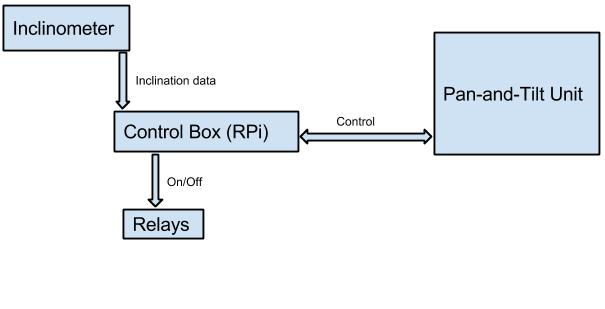
\includegraphics[width=0.8\linewidth]{model}
\captionof{figure}{Connection model}
\label{fig:model}
\end{center}
The figure~\ref{fig:model} shows the connection method that was chosen to interconnect all parts. At the moment inclinometer and relays work fine and are ready for the integration into the overall system. Currently work is undertaken to extend and improve functionality of the TASS protocol which is used to interact with the PTU. The control box which consists of raspberry pi has functionality to interact with the inclinometer and relays, as well as responds to the connected client commands.
\end{multicols}
}

%----------------------------------------------------------------------------------------
%	REFERENCES
%----------------------------------------------------------------------------------------

\headerbox{References}{name=references,column=0,above=bottom}{

\renewcommand{\section}[2]{\vskip 0.05em} % Get rid of the default "References" section title
\nocite{*} % Insert publications even if they are not cited in the poster
\small{ % Reduce the font size in this block
\bibliographystyle{unsrt}
\bibliography{bibl}
}}

%----------------------------------------------------------------------------------------
%	FUTURE RESEARCH
%----------------------------------------------------------------------------------------

\headerbox{Futher Research}{name=futureresearch,column=1,span=2,aligned=references,above=bottom}{ % This block is as tall as the references block
In future alternative methods will be researched to allow stabilization with less hardware overhead.
}

%----------------------------------------------------------------------------------------
%	CONTACT INFORMATION
%----------------------------------------------------------------------------------------

\headerbox{Contact Information}{name=contact,column=3,aligned=references,above=bottom}{ % This block is as tall as the references block

\begin{description}\compresslist
\item[Web] www.aber.ac.uk/PTU
\item[Email] IvanovEgdar@gmail.com
\item[Phone] 0753 114 2133
\end{description}
}

%----------------------------------------------------------------------------------------
%	CONCLUSION
%----------------------------------------------------------------------------------------

\headerbox{Conclusion}{name=conclusion,column=2,span=2,row=0,below=results,above=references}{
At the moment there are separate working parts. There is still much to do. The PTU TASS protocol needs to be improved to allow additional functionality. The main part of the application, which makes calculations based on data from the PTU and inclinometer, is still to be written.    

}

%----------------------------------------------------------------------------------------
%	MATERIALS AND METHODS
%----------------------------------------------------------------------------------------

\headerbox{Materials \& Methods}{name=method,column=0,below=objectives,bottomaligned=conclusion,span=2}{ % This block's bottom aligns with the bottom of the conclusion block

For this project I adapted Feature Driven Development methodology. It has been chosen because it will allow to deliver tangible, working software repeatedly in a timely manner at each stage of the project. \linebreak

At the initial stage of the project consultations with the project supervisor were conducted to understand the root of the problem. Possible solutions, including advantages and disadvantages, were discussed and shaped in the further meetings. \linebreak

Further research was made to understand the problems with gyroscopes and why they fail to provide accurate information. PTU data sheets and manuals were examined to find the path for possible solutions. 
}

\end{poster}

\end{document}